
\documentclass[10pt]{scrreprt} % Default font size and left-justified equations
\KOMAoptions{parskip=half}

\usepackage[top=2cm,bottom=2cm,inner=1cm,outer=1cm, a4paper]{geometry} % Page margins

\usepackage{xcolor, colortbl} % Required for specifying colors by name
\definecolor{bleu}{RGB}{0,102,204} % Define the blue color used for highlighting throughout the book
\definecolor{mygreen}{rgb}{0,0.6,0}
\definecolor{mygray}{rgb}{0.5,0.5,0.5}
\definecolor{mymauve}{rgb}{0.58,0,0.82}

\usepackage[french]{babel}  % French language
\DecimalMathComma
\usepackage[bitstream-charter]{mathdesign}

% Index
\usepackage{calc} % For simpler calculation - used for spacing the index letter headings correctly
\usepackage{makeidx} % Required to make an index
\makeindex % Tells LaTeX to create the files required for indexing

\usepackage{markdown}
%----------------------------------------------------------------------------------------
%	VARIOUS REQUIRED PACKAGES
%----------------------------------------------------------------------------------------
\usepackage{amsmath,amsfonts,amsthm} % For math equations, theorems, symbols, etc
\usepackage{esint}
\usepackage{siunitx}
\sisetup{locale = FR,inter-unit-product =\cdot}
\usepackage{titlesec} % Allows customization of titles

\usepackage{graphicx} % Required for including pictures
\usepackage{rotating}
\usepackage{wrapfig}
\usepackage{caption}
\usepackage{subcaption}
\usepackage{tabularx}

\usepackage{diagbox}

\usepackage{array}
\newcommand{\PreserveBackslash}[1]{\let\temp=\\#1\let\\=\temp}
\newcolumntype{C}[1]{>{\PreserveBackslash\centering}m{#1}}
\newcolumntype{R}[1]{>{\PreserveBackslash\raggedleft}m{#1}}
\newcolumntype{L}[1]{>{\PreserveBackslash\raggedright}m{#1}}


\graphicspath{./Pictures/} % Specifies the directory where pictures are stored
\renewcommand{\thefigure}{\arabic{section}.\arabic{figure}}
\renewcommand{\thetable}{\arabic{section}.\arabic{table}}

\usepackage{tikz} % Required for drawing custom shapes
\usetikzlibrary{trees,arrows,patterns,plotmarks, positioning}
\usepackage{forest}

\usepackage{pgfplots}
\usepackage{pgfplotstable}
\pgfplotsset{compat=1.10}
\usepgfplotslibrary{fillbetween}

\usepackage{enumitem} % Customize lists
\usepackage[f]{esvect}

\setlist{itemsep=1pt,topsep=1pt} % Reduce spacing between bullet points and numbered lists
\setitemize{label=\textbullet}

\usepackage{booktabs} % Required for nicer horizontal rules in tables

\usepackage{eso-pic} % Required for specifying an image background in the title page

\usepackage{multicol,multirow}
\usepackage{filecontents}

\usepackage{float}

%---------------
% 	 CODE
%---------------
\usepackage{minted}
\usepackage{tcolorbox}
\tcbuselibrary{listings, minted, skins}

\newfloat{lstfloat}{htbp}{lop}
\floatname{lstfloat}{Listing}
\def\lstfloatautorefname{Listing}

\tcbset{listing engine=minted}
\usemintedstyle[python]{tango}
\usemintedstyle[pycon]{tango}
\setmintedinline[python]{fontsize = \small}
\newcommand{\pyinline}[1]{\mintinline{python}{#1}}

\newtcblisting{pythonlst}{	listing only, minted language=python,
	sharp corners,
	width=10cm,
	minted options={%fontfamily=jkptt, 
		fontsize=\footnotesize, tabsize=2, breaklines, autogobble}, enhanced,frame hidden, 
	overlay unbroken and last={%
		\draw[line width=1mm, gray] (interior.north west)++(0,-0.25cm)   -- (interior.north west)-- (interior.north east)-- ++(0,-0.25cm) ;
		\draw[line width=1mm, gray] (interior.south west)++(0,0.25cm)   -- (interior.south west)-- (interior.south east)-- ++(0,0.25cm) ;}}

\newtcbinputlisting{\inputPython}[3]{listing file={#1},
	listing only, minted language=python,
	sharp corners,
	width=10cm,
	minted options={firstline=#2,lastline=#3,linenos, %fontfamily=jkptt, 
		fontsize=\footnotesize, tabsize=2, breaklines, autogobble}, enhanced,frame hidden, 
	overlay unbroken and last={%
		\draw[line width=1mm, gray] (interior.north west)++(0,-0.25cm)   -- (interior.north west)-- (interior.north east)-- ++(0,-0.25cm) ;
		\draw[line width=1mm, gray] (interior.south west)++(0,0.25cm)   -- (interior.south west)-- (interior.south east)-- ++(0,0.25cm) ;}}


\usepackage[noend]{algpseudocode}
\algrenewcommand\algorithmicwhile{\texttt{while}}
\algrenewcommand\algorithmicdo{\texttt{do}}
\algrenewcommand\algorithmicif{\texttt{if}}
\algrenewcommand\algorithmicthen{\texttt{then}}
\algrenewcommand\algorithmicelse{\texttt{else}}
\algnewcommand\Skip{\texttt{skip}}%	

%----------------------------------------------------------------------------------------
%	HYPERLINKS IN THE DOCUMENTS
%----------------------------------------------------------------------------------------

% For an unclear reason, the package should be loaded now and not later
\usepackage{hyperref}
\hypersetup{
	colorlinks,
	linkcolor={red!50!black},
	citecolor={blue!50!black},
	urlcolor={blue!80!gray}
}

%----------------------------------------------------------------------------------------
%	SECTION NUMBERING
%----------------------------------------------------------------------------------------
\setcounter{tocdepth}{3}
\setcounter{secnumdepth}{3}
\renewcommand\thesection{\arabic{section}}
\renewcommand\thesubsection{\arabic{section}.\arabic{subsection}}
\renewcommand\thesubsubsection{\arabic{section}.\arabic{subsection}.\arabic{subsubsection}}

%-------Set parskip for minipages--------
\makeatletter 
\let\org@parboxrestore\@parboxrestore 
\def\@parboxrestore{% 
  \edef\restore@parsettings{% 
    \parindent=\the\parindent\relax 
    \parskip=\the\parskip\relax 
  }% 
  \org@parboxrestore 
  \restore@parsettings 
} 
\makeatother 
 % Insert the commands.tex file which contains the majority of the structure behind the template

%equations sur plusieurs lignes, avec ou sans accolades
\newcommand\meq[1]{\begin{equation*}\begin{split}#1\end{split}\end{equation*}}
\newcommand\meqa[1]{\begin{equation*}\left\{\begin{split}#1\end{split}\right.\end{equation*}}

%Vecteurs (bases, opérateurs,...)
\newcommand\ux{\vv{u}_x}
\newcommand\uy{\vv{u}_y}
\newcommand\uz{\vv{u}_z}
\newcommand\ur{\vv{u}_r}
\newcommand\ut{\vv{u}_\theta}
\newcommand\uf{\vv{u}_\varphi}

\newcommand\ve[1]{\vv{#1}}

\newcommand\grad{\ve{\mathrm{grad}\,}}
\newcommand\dive{\mathrm{div}\,}
\newcommand\rot{\ve{\mathrm{rot}}\,}

%Opérateurs différentiels
\newcommand\dt[1]{\dfrac{\mathrm d #1}{\mathrm d t}}
\newcommand\ddt[1]{\dfrac{\mathrm d^2 #1}{\mathrm d t^2}}
\newcommand\Dt[1]{\dfrac{\mathrm D #1}{\mathrm D t}}

\newcommand\de {\mathrm d}
\newcommand\De {\mathrm D}

\newcommand\diff[2]{\dfrac{\mathrm d #1}{\mathrm d #2}}
\newcommand\pdiff[2]{\dfrac{\partial #1}{\partial #2}}

\newcommand\ddiff[2]{\dfrac{\mathrm d^2 #1}{\mathrm d #2^2}}
\newcommand\pddiff[2]{\dfrac{\partial^2 #1}{\partial #2^2}}

%unités
\newcommand\un[1]{\mathrm{\, #1}}


\title{UPSimulator}
\author{Maxence KLEIN\\ \and Véronique REYNAUD\\ \and Guillaume DESJOUIS }
\date{2020}

\begin{document}
\maketitle
\tableofcontents
\clearpage

\section{Présentation générale du projet}
\subsection{Objectifs}
Le projet \textsc{UPSimulator} a pour objectif de développer un simulateur de processeur à visée pédagogique. Celui-ci doit permettre d'appréhender la chaine conduisant d'un programme écrit dans un langage de haut niveau au détail de l'exécution à l'échelle du processeur. Pour cela, le projet doit permettre:
\begin{itemize}
	\item la production d'un code source dans un langage jouet;
	\item la compilation du code source et la production d'une version assembleur et binaire de celui-ci. Le simulateur doit permettre l'usage de différents modèles (taille des mots binaires, nombre de registre, ...);
	\item le suivi de l'exécution (registres, mémoire, pointeur, appels à l'UAL,...);
\end{itemize}

Les choix techniques retenus pour chaque fonctionnalité sont développés ci-après.

\begin{figure}[h!]
	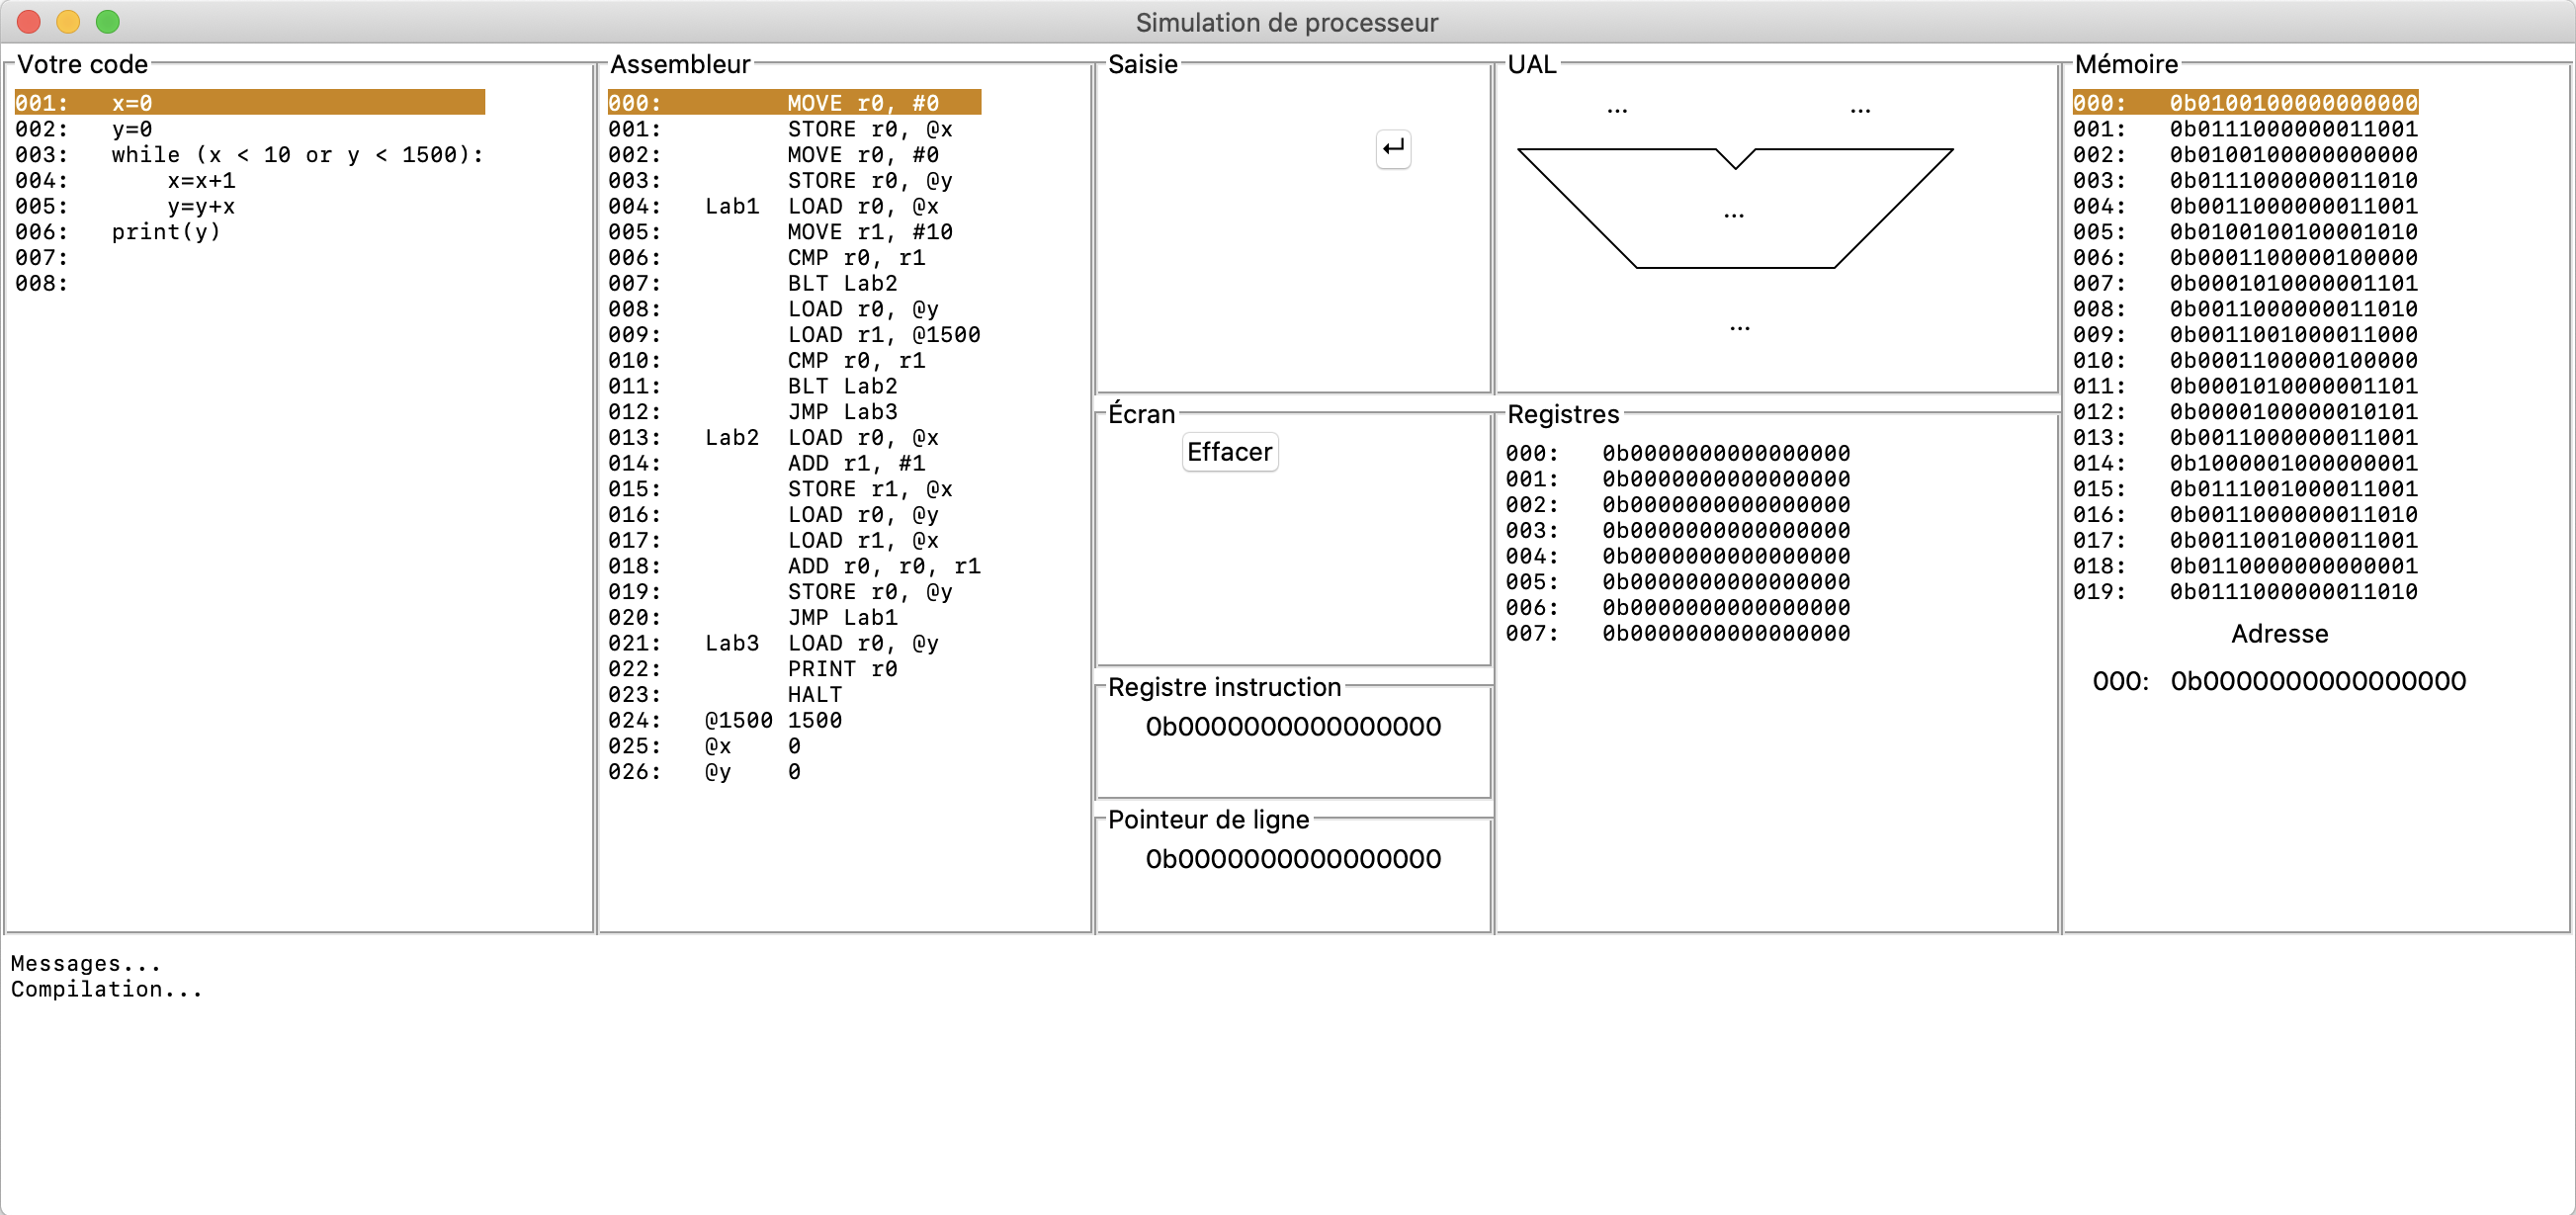
\includegraphics[width=\textwidth]{./Pictures/Header.png}
	\caption{\label{fig:gui} Interface Graphique}
\end{figure}
\subsection{Structure}
diag UML ou équivalent

\clearpage
\section{Choix techniques}
\subsection{Langage jouet}

Le langage jouet doit permettre à l'utilisateur de produire un exemple de code simple reprenant les principales structures (boucles, branchements conditionnels,...)

\begin{lstfloat}[h!]
	\centering
\inputPython{example2.code}{1}{11}
\caption{Exemple de code dans le langage jouet}
\end{lstfloat}

\subsubsection{Expressions admissibles}

Les expression admissibles sont présentées dans la table  \ref{tab:expressions} ci-dessous.
\begin{table}[h!]\caption{\label{tab:expressions}Expressions admissibles}
	\centering
	\begin{tabular}{|c|c|c|}
	\hline
	\multicolumn{2}{|c|}{Variable}   &            \pyinline{x}            \\ \hline
	\multicolumn{2}{|c|}{Entier}     &            \pyinline{n}            \\ \hline
	              &      Somme       &         \pyinline{e1 + e2}         \\ \cline{2-3}
	              &    Différence    &         \pyinline{e1 - e2}         \\ \cline{2-3}
	 Opérations   &     Produit      &         \pyinline{e1 * e2}         \\ \cline{2-3}
	arithmétiques & Division entière &         \pyinline{e1 / e2}         \\ \cline{2-3}
	              &      Reste       & \pyinline{e1 % e2
	              } \\ \cline{2-3}
	              &      Opposé      &           \pyinline{-e1}           \\ \hline
\end{tabular}
\hspace{3cm}
\begin{tabular}{|c|c|c|}
	\hline
	\multicolumn{3}{|c|}{Opérations logiques}                                         \\ \hline
	\multirow{10}{*}{Binaires} &           Egalité           &  \pyinline{e1 == e2}   \\ \cline{2-3}
	                           &         Différence          &  \pyinline{e1 != e2}   \\ \cline{2-3}
	                           & \multirow{4}{*}{Inégalités} &   \pyinline{e1 < e2}   \\ \cline{3-3}
	                           &                             &   \pyinline{e1 > e2}   \\ \cline{3-3}
	                           &                             &  \pyinline{e1 <= e2}   \\ \cline{3-3}
	                           &                             &  \pyinline{e1 >= e2}   \\ \cline{2-3}
	                           &     \multirow{2}{*}{Et}     &  \pyinline{e1 and e2}  \\ \cline{3-3}
	                           &                             &  \pyinline{e1 \& e2}   \\ \cline{2-3}
	                           &     \multirow{2}{*}{Ou}     &  \pyinline{e1 or e2}   \\ \cline{3-3}
	                           &                             & \pyinline{e1     | e2} \\ \hline
	 \multirow{2}{*}{Unaire}   &      inverse bit à bit      &     \pyinline{~e1}     \\ \cline{2-3}
	                           &      négation logique       &   \pyinline{not e1}    \\ \hline
\end{tabular}
\end{table}
%
\subsubsection{Liste de commandes admissibles}

\begin{minipage}[c]{0.38\textwidth}
	\begin{minted}[frame = single, label={Affectation}]{python}
x=e
\end{minted}
\end{minipage}
\hspace{1cm}
\begin{minipage}[c]{0.38\textwidth}
	avec \pyinline{e} une expression logique ou arithmétique.
\end{minipage}
\vspace{0.5cm}

\begin{minipage}[c]{0.38\textwidth}
\begin{minted}[frame = single, label={Branchement conditionnel}]{python}
if e :
	c1
elif e2: 
	c2
else:
	c3
\end{minted}
\end{minipage}
\hspace{1cm}
\begin{minipage}[c]{0.38\textwidth}
	avec \pyinline{e1} et \pyinline{e2} des expressions et \pyinline{c1}, \pyinline{c2} et \pyinline{c3} des commandes.
	
	Les branchement \pyinline{else} et \pyinline{elif} sont optionnels.
\end{minipage}
\vspace{0.5cm}

\begin{minipage}[c]{0.38\textwidth}
\begin{minted}[frame = single, label={Boucle}]{python}
while e :
	c1
\end{minted}
\end{minipage}
\hspace{1cm}
\begin{minipage}[c]{0.38\textwidth}
	avec \pyinline{e} une expression et \pyinline{c} une commande.	
\end{minipage}
\vspace{0.5cm}

\begin{minipage}[c]{0.38\textwidth}
\begin{minted}[frame = single, label={Lecture clavier}]{python}
input()
\end{minted}
\end{minipage}
\vspace{0.5cm}

\begin{minipage}[c]{0.38\textwidth}
\begin{minted}[frame = single, label={Ecriture sur la sortie courante}]{python}
print(v)
\end{minted}
\end{minipage}
\hfill
\begin{minipage}[c]{0.38\textwidth}
	avec \pyinline{e} une expression	
\end{minipage}

\subsubsection{Indentations}
Le code est indenté comme en python afin de détecter les blocs:
\begin{itemize}
	\item L'indentation n'augmente qu'après un \pyinline{:} lié à une structure \pyinline{if} ou \pyinline{while}
	\item L'indentation ne peut diminuer que atteindre un niveau précédemment atteint.
\end{itemize}

\subsubsection{Commentaires}
Les commentaires sont repérés par le caractère \pyinline{#} .

\begin{lstfloat}
	\begin{center}
	\begin{pythonlst}
aaaaaaaaaa:
	aaaaaaaaaa
	aaaaaaaaaa
		aaaaaaaaaa # pas valable il manque : avant
		aaaaaaaaaa
	aaaaaaaaaa
aaaaaaaaaa
aaaaaaaaaa:
			aaaaaaaaaa
	aaaaaaaaaa # pas valable. Ce niveau a été atteint avant mais pas dans le même bloc
aaaaaaaaaa
\end{pythonlst}
\caption{Langage jouet - Commentaires et indentations}
\end{center}
\end{lstfloat}





\clearpage

\subsection{Parsing}


\begin{minipage}[t]{0.7\textwidth}
	Une étape d'analyse du code (parsing) est nécessaire en amont de la production du code assembleur. Cette étape a pour objet:
\begin{itemize}
	\item d'assurer que la syntaxe du langage jouet est respectée
	\item de permettre la construction d'un arbre représentant les différentes structures du code source afin de pouvoir produire le code assembleur et le binaire associé
\end{itemize}
\end{minipage}
\hfill
\begin{minipage}[t]{0.3\textwidth}
	\vspace{-1.5cm}
	\centering
	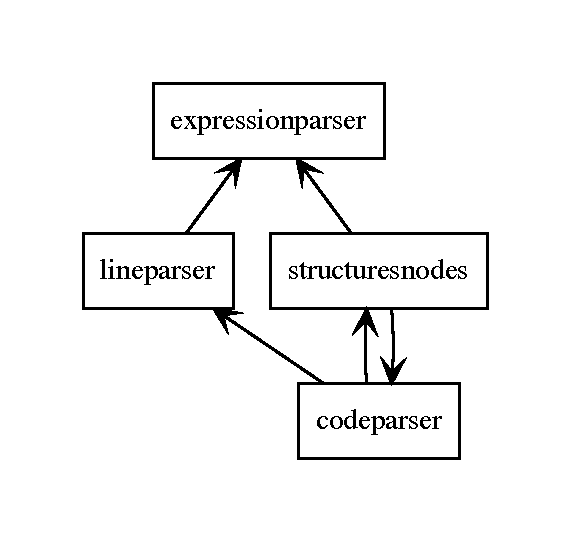
\includegraphics[scale=0.7]{./Pictures/parser.pdf}
	\captionof{figure}{}
\end{minipage}

\begin{figure}[h!]
	\centering
	\begin{tikzpicture}
	\node (ifelif) at (0,0) {
		\begin{minipage}{6cm}
		\inputminted[frame = single]{python}{example.code}
		\end{minipage}
	};
	
	
	\node[right = 4cm of ifelif.east] (ifelseif) {
\begin{minipage}{7.5cm}
\begin{minted}[frame = single]{text}
[<structuresnodes.AffectationNode >,
<structuresnodes.AffectationNode >,
<structuresnodes.WhileNode>,
<structuresnodes.PrintNode>]
\end{minted}
\end{minipage}
	};
	
	\draw[->] (ifelif.east) -- (ifelseif) node[midway, above] {\pyinline{CodeParser}};
	\end{tikzpicture}
	\caption{Exemple simpliste de parse}
\end{figure}


\subsubsection{Classe CodeParser}

L'analyse du code est gérée par un objet de la classe \pyinline{CodeParser} dont le constructeur prend en argument:
\begin{itemize}
	\item soit un nom de fichier \pyinline{filename = file}
	\item soit une chaine de caractère contenant un fragment de code \pyinline{code = fragment}
\end{itemize}

Un objet de type \pyinline{CodeParser} a pour attributs:
\begin{itemize}
	\item \pyinline{__listingCode}: une liste d'objets de type \pyinline{LineParser}
	\item \pyinline{__structuredListeNode} un arbre d'objets de type StructureNode contenant le code interprété
\end{itemize}

Lorsque le code est donné sous forme de fichier, la méthode \pyinline{__parseFile} permet de récupérer la chaîne de caractères correspondante.

La méthode \pyinline{parseCode} construit une instance de la classe \pyinline{LineParser} pour chaque ligne de code source. Si la ligne n'est pas vide, les caractéristiques de celles-ci sont ajoutées à la liste \pyinline{__listingCode}.

Une analyse syntaxique succincte est réalisée avec l'appel successif aux méthodes:
\begin{itemize}
	\item  \pyinline{__manageElif}: réécriture des branchements \pyinline{elif}).
	\begin{center}

\begin{tikzpicture}
\node (ifelif) at (0,0) {
\begin{minipage}{3cm}
\begin{minted}[frame = single]{python}
if e1 :
	c1
elif e2 :
	c2
else c3
\end{minted}
\end{minipage}
};


\node[right = 5cm of ifelif.east] (ifelseif) {
\begin{minipage}{5cm}
\begin{minted}[frame = single]{python}
if e1 :
	c1
else :
	if e2 :
		c2
	else :
		c3
\end{minted}
\end{minipage}
};

\draw[->] (ifelif.east) -- (ifelseif) node[midway, above] {\pyinline{__manageElif}};
\end{tikzpicture}
		
	\end{center}
	\item \pyinline{__blocControl}: test de la syntaxe des structures de contrôle et de l'indentation associée.
\end{itemize}


Finalement, la construction de l'arbre \pyinline{__structuredListeNode} nécessite l'appel des méthodes:
\begin{itemize}
	\item \pyinline{__buildFinalNodeList()}: construit les n\oe uds (instances de classe \pyinline{structuresnodes}) et l'arborescence correspondante à partir des caractéristiques \pyinline{__listingCode}. Les blocs d'instructions sont ajoutés à \pyinline{__structuredListeNode}.
	
	\item \pyinline{__structureList}: Parcours du listing \pyinline{__listingCode} pour ranger les enfants et leur associer le bon niveau d'indentation
\end{itemize} 


L'arborescence des n\oe uds \pyinline{__listingCode} peut-être affichée à l'aide des méthodes des \pyinline{__str__} et \pyinline{__recursiveStringifyLine}.

L'accès à la liste de n\oe uds \pyinline{__structureList} est possible à l'aide de l'accesseur \pyinline{getFinalParse}.

\subsubsection{Classe LineParser}

La classe \pyinline{LineParser} permet de renvoyer les caractéristiques d'une ligne de code sous forme d'un dictionnaire contenant numéro de ligne, niveau d'indentation, caractère vide ou non, motif identifié (if,....), condition, expression ou variable le cas échéant.

Pour une ligne de code donnée elle doit:
\begin{itemize}
	\item Nettoyer le code des commentaires et espaces terminaux: \pyinline{__suppCommentsAndEndSpaces}
	\item Déterminer le niveau d'indentation: \pyinline{__countIndentation}
	\item Pour les lignes non vides, identifier le motif: \pyinline{__identificationMotif}
\end{itemize}

Lorsque le motif correspond à un branchement conditionnel \pyinline{if e} ou une boucle \pyinline{while e} l'identification du motif \pyinline{__identificationMotif} nécessite de tester que \pyinline{e} est une expression valide. L'expression correspondante est construite par une instance de la classe \pyinline{ExpressionParser}.


\subsubsection{Classe ExpressionParser}

Les objets de la classe \pyinline{ExpressionParser}  permettent l'interprétation d'une chaine de caractère afin de renvoyer un objet de type expression, c'est à dire un arbre dont chaque n\oe ud représente un opérateur binaire, un opérateur unaire, une variable ou un littéral.

Pour cela la chaine de caractère représentant l'expression est convertie en une liste de Tokens (\pyinline{__buildTokensList(cls, expression:str) }) représentant chaque type admissible dans la chaine de caractère

La classe doit permettre de vérifier la syntaxe de l'expression 


\subsection{Code Assembleur}
\subsection{Modèle de processeur}
\subsection{Interface utilisateur}
\subsection{Gestion de la documentation}
\section{Organisation}
\subsection{Planification}

\begin{figure}[h!]
	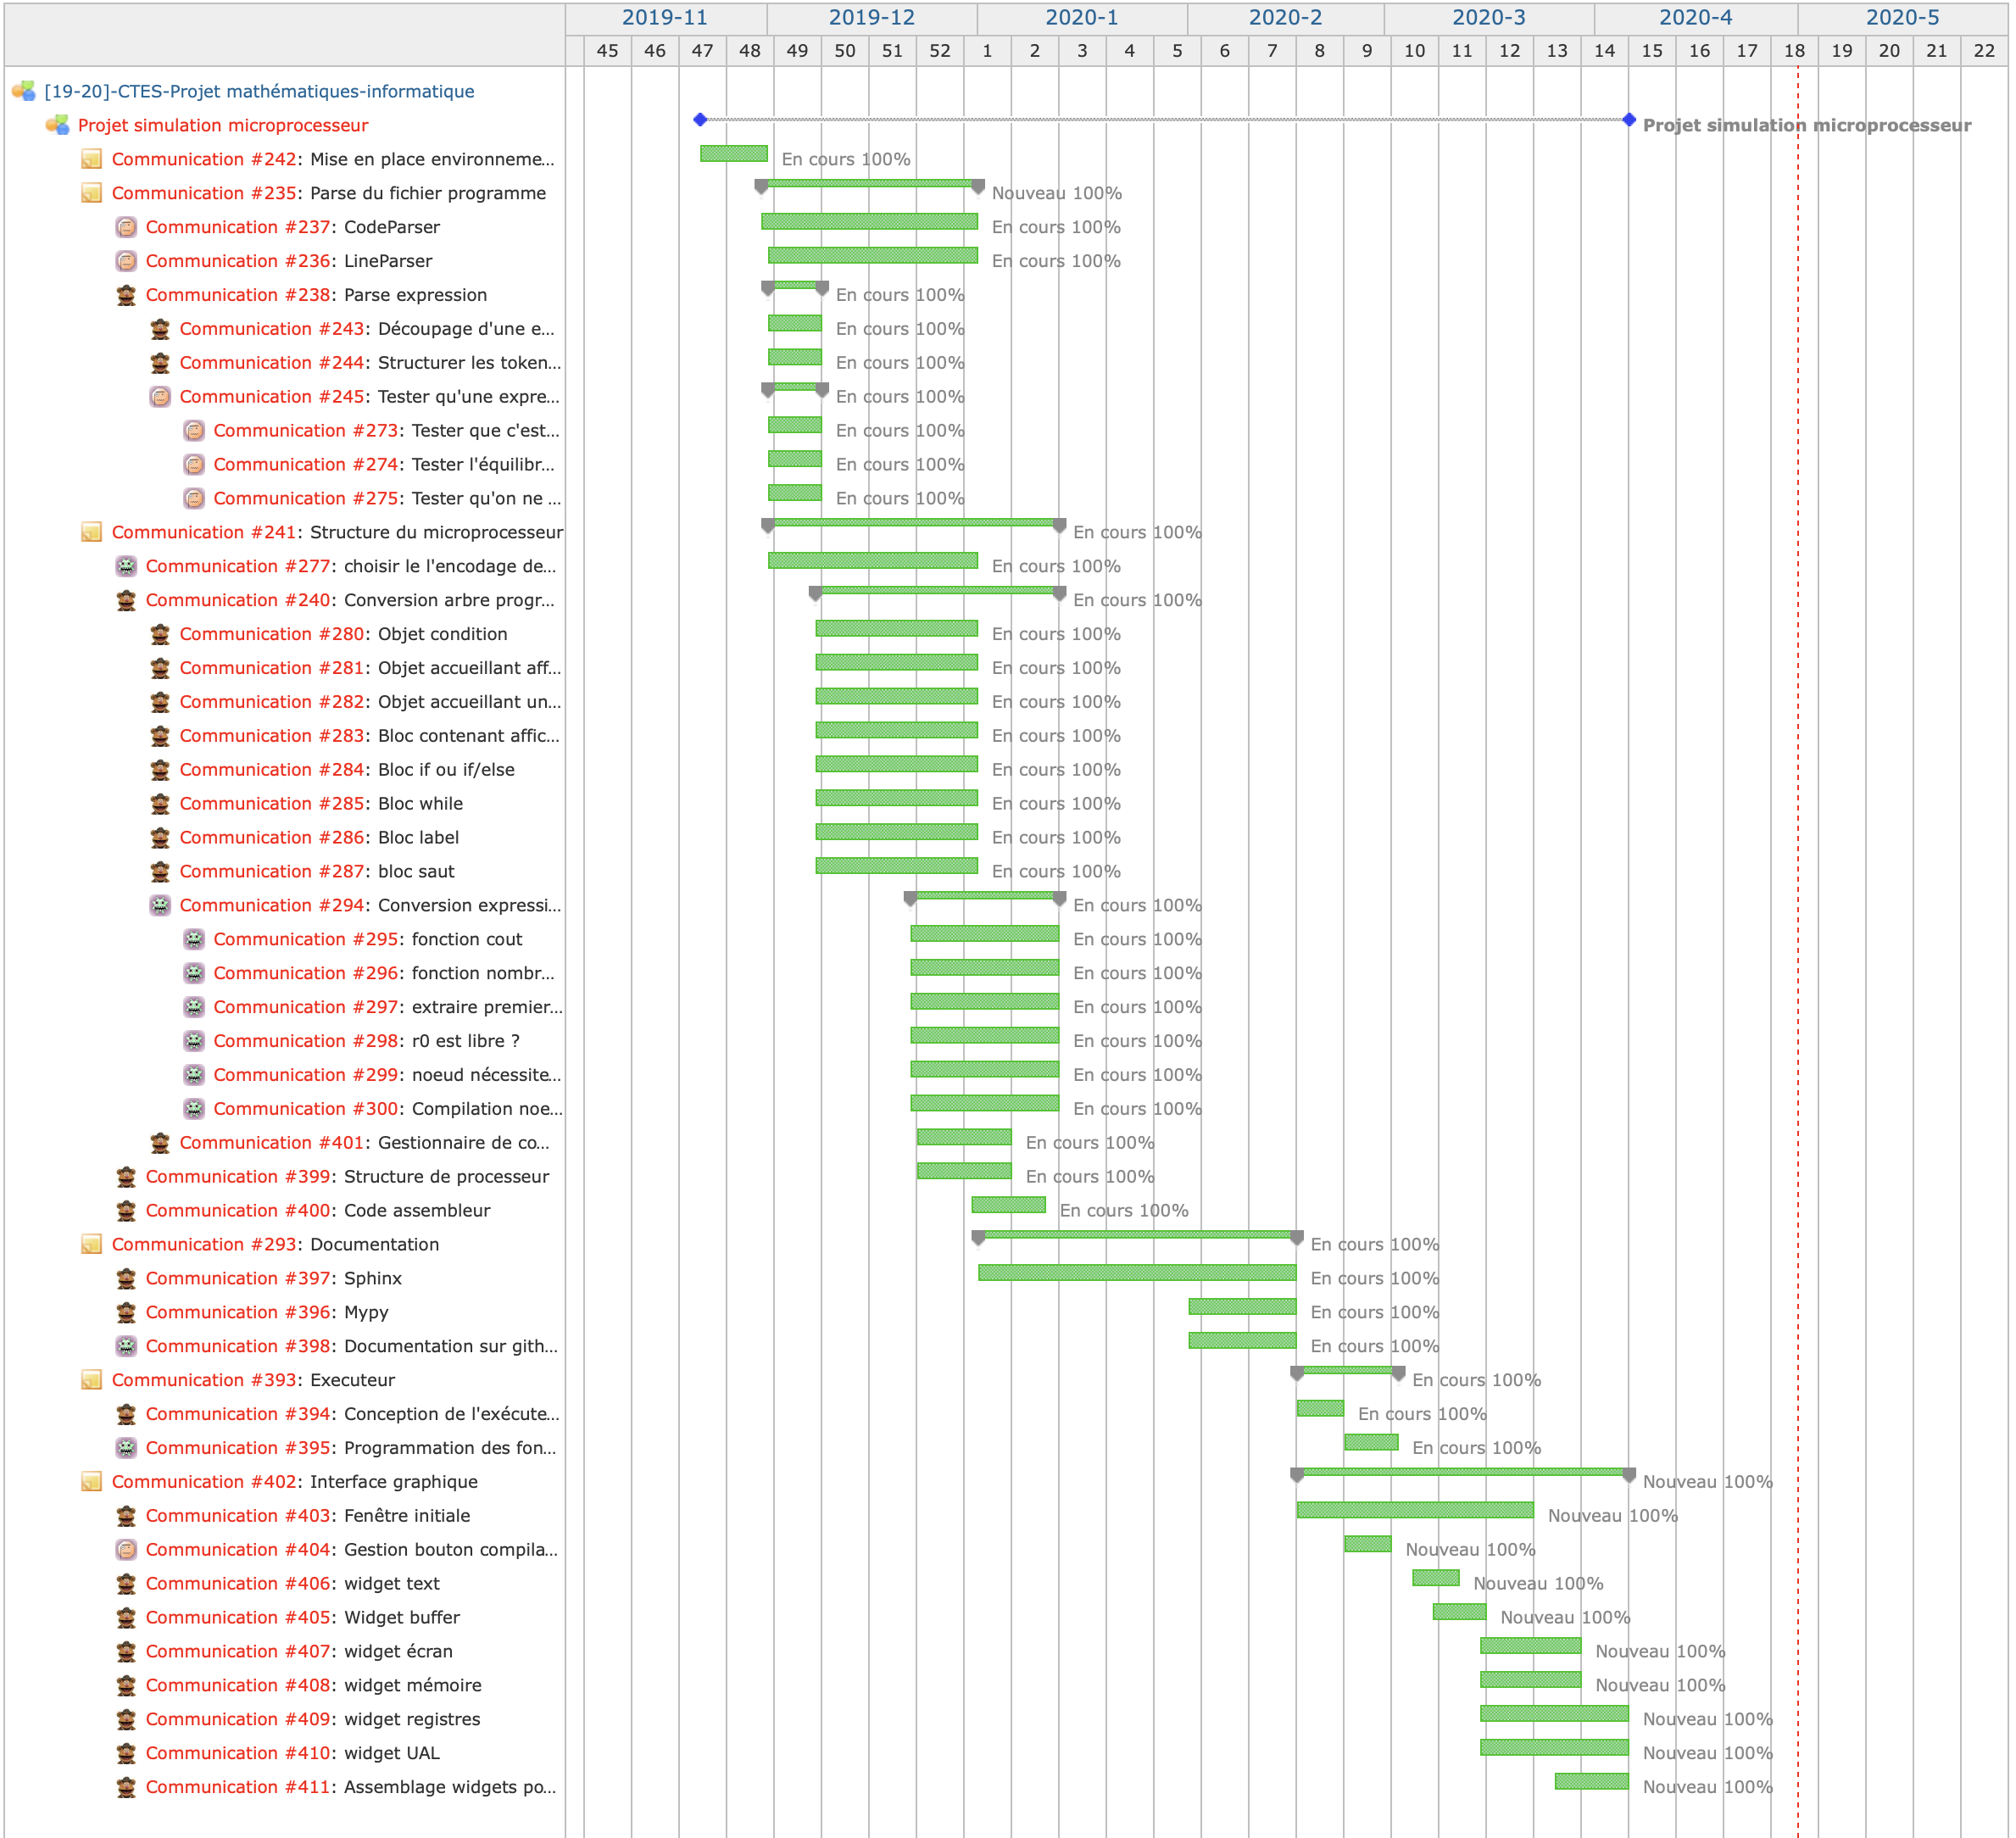
\includegraphics[width=\textwidth]{./Pictures/Gantt.png}
	\caption{Diagramme de Gantt du projet}
\end{figure}

\subsection{Répartition des tâches}
\begin{appendix}
	\listoffigures
	\listoftables
\end{appendix}

\end{document}